\documentclass[]{article}
\usepackage{amssymb}
\usepackage{amsmath}
\usepackage[utf8]{inputenc}
\usepackage{graphicx}
\usepackage{booktabs}
\usepackage{listings}
\usepackage{color}
\usepackage{tabularx}
\usepackage{hyperref}

\definecolor{dkgreen}{rgb}{0,0.6,0}
\definecolor{gray}{rgb}{0.5,0.5,0.5}
\definecolor{mauve}{rgb}{0.58,0,0.82}

\lstset{frame=tb,
	language=C++,
	aboveskip=3mm,
	belowskip=3mm,
	showstringspaces=false,
	columns=flexible,
	basicstyle={\small\ttfamily},
	numbers=none,
	numberstyle=\tiny\color{gray},
	keywordstyle=\color{blue},
	commentstyle=\color{dkgreen},
	stringstyle=\color{mauve},
	breaklines=false,
	breakatwhitespace=true,
	tabsize=2
}

%opening
\title{FYS4150 H20 Project 1}
\author{Olav Fønstelien}

\begin{document}

\maketitle

\begin{abstract}
In this assignment we investigate and compare three different algorithms for a numerical solution to Poisson's equation with Dirichlet boundary conditions on a domain $x \in \mathbb{R}$. The efficiency of the three algorithms are compared with regards to speed and memory. We will see that the efficiency of a purely library-based general algorithm for solving a system of linear equations is greatly surpassed when we take into account the tridiagonal character of the coefficient matrix; and that the efficiency is further increased when we take into account the fixed pattern of the diagonals in the equation. We will also see that the relative error of the numerical solution has a simple analytical representation which only depends on step size $h$. 

I have implemented the algorithms in C++ using the Armadillo library. See \lstinline|project1.cpp|, the \lstinline|Makefile| and a \lstinline|README.md| at my repository \url{https://github.com/fonstelien/FYS4150/tree/master/project1}.
\end{abstract}

\section*{A: Establishing the system of linear equations}
Poisson's equation is a second degree differential equation on the form $u''(x) = f(x, u(x))$, and the assignment already gives us the form of the numerical approximation $v_i \approx u_i$ to this problem as

\begin{equation}
\label{eqn:approx_2nd_der}
-\frac{v_{i-1} -2v_i + v_{i+1}}{h^2} = f_i \Rightarrow -v_{i-1} +2v_i - v_{i+1} = h^{2}f_i.
\end{equation}

With boundary values $u_0 = u(0) = \alpha$ and $u_{n+1} = u(1) = \beta$, we get the equations

\begin{align*}
-\alpha + 2v_1 - v_2 &= h^{2}f_1 \\
-v_1 + 2v_2 - v_3 &= h^{2}f_2 \\
&\vdots \\
-v_{n-1} + 2v_n -\beta &= h^{2}f_n.
\end{align*}

Now, with $\alpha = \beta = 0$ we can represent this as the set of linear equations $\mathbf{Av} = \mathbf{\tilde{b}}$ where $\mathbf{A} \in \mathbb{R}^{n \times n}$ is tridiagonal with diagonal weights $-1, 2$ and $-1$, $\mathbf{v} = \{v_1, v_2, \ldots, v_n\}$ ,and $\mathbf{\tilde{b}} = \{h^{2}f_1, h^{2}f_2, \ldots, h^{2}f_n\}$:

\begin{equation*}
\left[ \begin{matrix}
2 & -1 & 0 & \cdots & 0 \\
-1 & 2 & -1 & \ddots & \vdots \\
0 & \ddots & \ddots & \ddots & 0\\
\vdots & \ddots & -1 & 2 & -1 \\
0 & \cdots & 0 & -1 & 2
\end{matrix} \right]
\left[ \begin{matrix}
v_1 \\
v_2 \\
\vdots \\
v_n
\end{matrix} \right] = 
h^{2} \left[ \begin{matrix}
f_1 \\
f_2 \\
\vdots \\
f_n
\end{matrix} \right]
\end{equation*}



\section*{B: General numerical solution to a tridiagonal system of linear equations}
The first programming task is to find an algorithm for a solution to the general tridiagonal problem

\begin{equation*}
\mathbf{Av} = 
\left[ \begin{matrix}
b_1 & c_1 & 0 & \cdots & 0 \\
a_2 & b_2 & c_2 & \ddots & \vdots \\
0 & \ddots & \ddots & \ddots & 0 \\
\vdots & \ddots & a_{n-1} & b_{n-1} & c_{n-1} \\
0 & \cdots & 0 & a_n & b_n
\end{matrix} \right]
\left[ \begin{matrix}
v_1 \\
v_2 \\
\vdots \\
v_n
\end{matrix} \right] = 
\mathbf{\tilde{b}} = 
\left[ \begin{matrix}
\tilde{b}_1 \\
\tilde{b}_2 \\
\vdots \\
\tilde{b}_n
\end{matrix} \right] .
\end{equation*}

To solve this, let's first subtract $\frac{a_2}{b_1}$ times the first row from the second row in $\mathbf{A}$ to get rid of the first non-zero coefficient:


\begin{equation*}
\left[ \begin{array} {ccccc|c}
b_1 & c_1 & 0 & \cdots & 0 & \tilde{b}_1\\
0 & b_2 - \frac{a_2}{b_1}c_1 & c_2 & \ddots & \vdots & \tilde{b}_2 -\frac{a_2}{b_1}\tilde{b}_1 \\
\vdots & \ddots & \ddots & \ddots & \vdots & \vdots \\
\end{array} \right].
\end{equation*}

We will denote these new values in the central diagonal and constant vector $b_{2}^{\ast} = b_2 - \frac{a_2}{b_1}c_1$ and $\tilde{b}_{2}^{\ast} = \tilde{b}_2 - \frac{a_2}{b_1}\tilde{b}_1$, with the general terms

\begin{equation*}
\begin{aligned}
b_{i}^{\ast} &= b_i - \frac{a_i}{b_{i-1}}c_{i-1} \\
\tilde{b}_{i}^{\ast} &= \tilde{b}_i - \frac{a_i}{b_{i-1}}\tilde{b}_{i-1}
\end{aligned}
\qquad \text{, for } i = 1,2,...,n \text{.}
\end{equation*}

Forward substitution of the rest of the rows will then give us $v_n$:

\begin{equation*}
\left[ \begin{array} {cccccc|c}
b_1 & c_1 & 0 & \cdots & & 0 & \tilde{b}_1\\
0 & b_{2}^{\ast} & c_2 & \ddots & & \vdots & \tilde{b}_{2}^{\ast} \\
\vdots & \ddots & b_{3}^{\ast} & \ddots & & & \tilde{b}_{3}^{\ast} \\
& & & \ddots & & & \vdots \\
& & & & b_{n-1}^{\ast} & c_{n-1} & \tilde{b}_{n-1}^{\ast} \\
& & & & 0 & b_{n}^{\ast} & \tilde{b}_{n}^{\ast}
\end{array} \right]
\Rightarrow v_n = \tilde{b}_{n}^{\ast} / b_{n}^{\ast} = \tilde{b}_{n}^{\ast\ast}.
\end{equation*}

Now that we have found $v_n$, finding the rest is easy. First we find $v_{n-1} = \tilde{b}_{n-1}^{\ast} - c_{n-1}\tilde{b}_{n}^{\ast\ast} = \tilde{b}_{n-1}^{\ast\ast}$, and then the remaining $v_i$ in the same manner:

\begin{equation*}
\left[ \begin{matrix}
1 & 0 & \cdots & 0 \\
0 & 1 & \ddots & \vdots \\
\vdots & \ddots & \ddots & 0\\
0 & \cdots & 0 & 1 \\
\end{matrix} \right]
\left[ \begin{matrix}
v_1 \\
v_2 \\
\vdots \\
v_n
\end{matrix} \right] = 
\left[ \begin{matrix}
\tilde{b}_{1}^{\ast\ast} \\
\tilde{b}_{2}^{\ast\ast} \\
\vdots \\
\tilde{b}_{n}^{\ast\ast}
\end{matrix} \right]
\end{equation*}

Counting the number of FLOPs needed to solve the tridiagonal $\mathbf{Av} = \mathbf{\tilde{b}}$ problem, we see that updating each term in the forward substitution process requires one division, one multiplication and one subtraction, and that we must do this $n-1$ times; that is $N_{\text{fwd}} = 2 \times 3 \times (n-1) = 6(n-1)$. Solving for $x_n$ requires one operation, and backward substitution to solve for remaining $n-1$ requires 3 operations each, giving $N_{\text{bwd}} = 1 + 3 \times (n-1) \approx 3(n-1)$ operations. All in all, the required number of FLOPs for a system of size $n$ is

\begin{equation*}
N_{\text{tridiag}} = N_{\text{fwd}} + N_{\text{bwd}} = 9(n-1).
\end{equation*}

We should note that the above algorithm allows us to reuse the space which originally contained the description of the problem; that is $\mathbf{A}$ and $\mathbf{\tilde{b}}$; amd also that we have found an algorithm which will solve a set of $n$ equation in $\mathcal{O}(n)$ time. This means that it is objectively efficient and scales well. You will find my C++ implementation of this algorithm in \lstinline|solve_tridiagonal()|. 

Let's move on and compare how the numerical approximation given in equation \ref{eqn:approx_2nd_der} performs relative to the closed-form solution. The assignment gives us the functions $f$ and the closed-form solution $u$ to the differential equation:

\begin{align*}
f(x) &= 100e^{-10x} \\
u(x) &= 1 - (1 - e^{-10})x - e^{-10x}.
\end{align*}

We insert $f_i = f(x_i) = f(hi)$ into our numerical approximation for various step sizes $h$ and observe from the plotted results in Figure \ref{fig:calc-results} below that the approximation $v_i$ approaches $u_i$ for decreasing $h$, as expected.

\begin{figure}[t]
	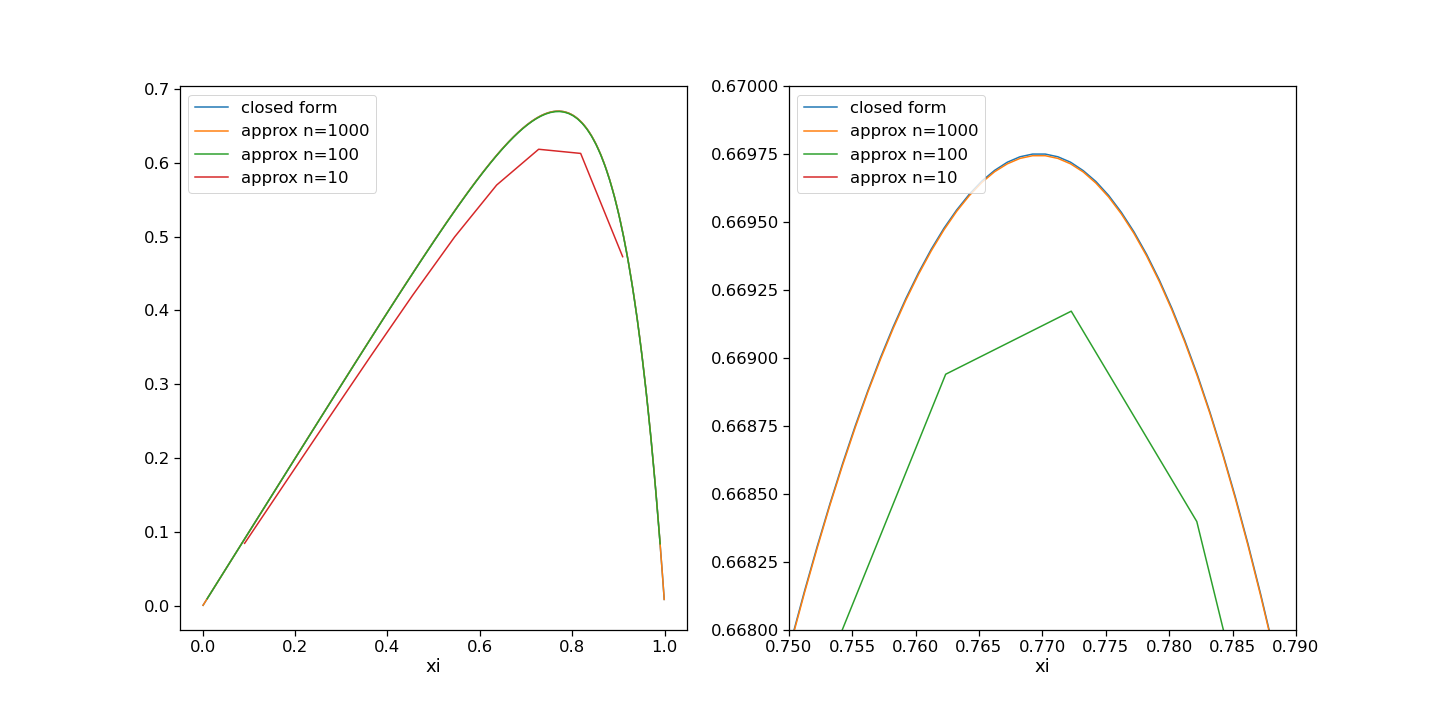
\includegraphics[width=1.2\linewidth]{calc-results.png}
	\caption{Plot of the numerical solution to the Poisson equation vs the closed-form solution. When $n > 100$ we see that the numerical solution is very close to the closed-form.}
	\label{fig:calc-results}
\end{figure}

\section*{C: Optimized numerical solution to the Poisson equation $-u''(x) = f(x)$}
Let's now take into consideration the fixed form of the diagonals of the coefficient matrix

\begin{equation*}
\mathbf{A} = 
\left[ \begin{matrix}
2 & -1 & 0 & \cdots & 0 \\
-1 & 2 & -1 & \ddots & \vdots \\
0 & \ddots & \ddots & \ddots & 0\\
\vdots & \ddots & -1 & 2 & -1 \\
0 & \cdots & 0 & -1 & 2
\end{matrix} \right]\text{.}
\end{equation*}

In contrast to the general case solved in Section B, this time we know everything there is to know about $\mathbf{A}$, and the solution will only be dependent on the constant vector $\mathbf{\tilde{b}}$. As soon as we have found out which steps are needed to transform $\mathbf{A}$ to $\mathbf{I}$, we can concentrate only on operations on $\mathbf{\tilde{b}}$, which will yield an algorithm which is optimized both with regards to speed and memory.

To find the solution, we first multiply row 2 with 2 and add row 1:

\begin{equation*}
\left[ \begin{array} {ccccc|c}
2 & -1 & 0 & \cdots & 0 & \tilde{b}_1\\
0 & 3 & -2 & \ddots & \vdots & 2\tilde{b}_2 + \tilde{b}_1\\
0 & -1 & 2 & -1 & \vdots & \tilde{b}_3\\
\vdots & \ddots & \ddots & \ddots & \vdots & \vdots \\
\end{array} \right].
\end{equation*}

We now see that to get rid of $a_3 = -1$ in the next row, we must this time multiply row 3 with 3 and add row 2, which will mean that in row 4 we must multiply with 4, and so on until we get $[\mathbf{A}|\mathbf{\tilde{b}}]$ on the wanted form, and we can solve for $v_n$:

\begin{equation*}
\left[ \begin{array} {ccccccc|c}
2 & -1 & 0 & \cdots & & & 0 & \tilde{b}_1\\
0 & 3 & -2 & \ddots & & & \vdots & \tilde{b}_{2}^{\ast}\\
\vdots & \ddots & 4 & -3 & & & & \tilde{b}_{3}^{\ast}\\
& & & \ddots & \ddots &&  \vdots& \vdots\\
&&&&&&&\\
\vdots & & & & \ddots & n & -(n-1) & \tilde{b}_{n-1}^{\ast}\\
0 & \cdots & & & & 0 & n+1 & \tilde{b}_{n}^{\ast}\\
\end{array} \right]
\Rightarrow v_n = \tilde{b}_{n}^{\ast} / (n+1).
\end{equation*}

Here we have denoted the new values in the constant vector $\mathbf{\tilde{b}}$ as $\tilde{b}_{2}^{\ast} = 2\tilde{b}_2 - \tilde{b}_1$,
$\tilde{b}_{3}^{\ast} = 3\tilde{b}_3 - \tilde{b}_{2}^{\ast}$, with the general term:

\begin{equation*}
\tilde{b}_{i}^{\ast} = i\tilde{b}_{i} + \tilde{b}_{i-1}^{\ast}
\end{equation*}

We now find $x_{n-1} = \frac{1}{n}(\tilde{b}_{n-1}^{\ast} + (n-1)\tilde{b}_{n}^{\ast}) = \tilde{b}_{n-1}^{\ast\ast}$, and again on general form $x_i = \frac{1}{i+1}(\tilde{b}_{i}^{\ast} + i\tilde{b}_{i+1}^{\ast}) = \tilde{b}_{i}^{\ast\ast}$, which gives us the solution

\begin{equation*}
\mathbf{v} = \mathbf{\tilde{b}^{\ast\ast}}\text{.}
\end{equation*}

As mentioned above, this algorithm is optimized both with regards to speed and memory. Memory required to solve a given problem is limited to the memory needed to describe it. Counting the FLOPs, we see that since we know how the forward substitution will unfold, each $n-1$ rows require one multiplication and one addition, and $N_{\text{fwd}} = 2(n-1)$. Likewise for backward substitution, we only need one multiplication, one addition, and one division, and $N_{\text{bwd}} = 3(n-1)$. In total, the number of FLOPs required for a system of size $n$ is

\begin{equation*}
N_{\text{Poisson}} = N_{\text{fwd}} + N_{\text{bwd}} = 5(n-1).
\end{equation*}

Compared to the general case discussed in Section B, this of course is quite good, but the real benefit comes from the greatly decreased memory use. Numerical problems such as these are usually memory-bound, not CPU bound. We see that general triagonal system required three vectors $\mathbf{a},\mathbf{b},\mathbf{c}$ for the coefficients and a fourth $\mathbf{\tilde{b}}$ for the constants which must all be streamed from main memory, or at least Level 3 cache for a system of some size. The optimized Poisson system, however, only needs the constant vector $\mathbf{\tilde{b}}$, and therefore requires far fewer reads and writes for solving the system. This is the reason for the approximately 2.5-3 times speedup that we see in Table \ref{tab:CPU-times} below.


\begin{table}[ht]
\caption{CPU time needed to solve the Poisson equation. The algorithm optimized for the Poisson equation has better speedup than expected from counting the FLOPs. The reason is fewer read/write operations.}
\label{tab:CPU-times}
\begin{center}
\begin{tabular}{lrrr}
	\toprule
	n &  General time [ms] &  Optimized time [ms] & Speedup factor \\
	\midrule
	100     &    0.103 &    0.042 &  2.452381 \\
	1000    &    0.659 &    0.277 &  2.379061 \\
	10000   &   10.179 &    3.385 &  3.007090 \\
	100000  &   55.765 &   20.122 &  2.771345 \\
	1000000 &  459.470 &  189.190 &  2.428617 \\
	\bottomrule
\end{tabular}
\end{center}
\end{table}


\section*{D: Relative error of the numerical solution to the Poisson equation}
Given the closed-form solution $u(x)$ to the Poisson equation $-u''(x) = f(x)$, we can calculate the relative error of our approximation $v_i$ to $u_i$:

\begin{equation*}
\varepsilon_{i} = \Bigl \lvert \frac{v_i - u_i}{u_i} \Bigr \rvert \text{.}
\end{equation*}

If we calculate this value for a sample of $i$, we will quickly notice that for a given step size $h$, $\varepsilon_i$ seems to be constant. To investigate this further, let's assume for a moment that indeed it \textit{is} constant, such that $\varepsilon_i = \varepsilon$, and

\begin{equation*}
\varepsilon = \Bigl \lvert \frac{v_{i-1} - u_{i-1}}{u_{i-1}} \Bigr \rvert = \Bigl \lvert \frac{v_{i} - u_{i}}{u_{i}} \Bigr \rvert = \Bigl \lvert \frac{v_{i+1} - u_{i+1}}{u_{i+1}} \Bigr \rvert \Rightarrow \begin{cases}
v_{i-1} &= u_{i-1}(1+\varepsilon) \\
v_{i} &= u_{i}(1+\varepsilon) \\
v_{i+1} &= u_{i+1}(1+\varepsilon)
\end{cases} \text{.}
\end{equation*}

If we install this for $v_{i-1},v_{i},v_{i+1}$ in the numerical approximation $2v_i - v_{i-1} - v_{i+1} = h^{2}f_i$, we get that the relative error is given as

\begin{equation*}
\varepsilon = \Biggl \lvert 1+ \frac{h^{2}f_i}{2u_i - u_{i-1} - u_{i+1}} \Biggr \rvert \text{.}
\end{equation*}

Now, with $f_i = f(ih) = 100e^{-10ih}$ and $u_i = u(ih) = 1 - (1 - e^{-10})ih - e^{-10ih}$, we get an expression for $\varepsilon$ that is independent of $i$, meaning that the relative error is indeed constant for any step size $h$:

\begin{equation}
\begin{split}
\label{eqn:eps-math}
\varepsilon = 1+ \frac{h^{2} \cdot 100e^{-10ih}}{2e^{-10ih} - e^{-10(i-1)h} - e^{-10(i+1)h}} &= 1+ \frac{100h^{2}}{2 - e^{10h} - e^{-10h}} \\&= 1 - \frac{50h^2}{\cosh 10h - 1} \text{.}
\end{split}
\end{equation}

It is also interesting to see what happens as $h \rightarrow 0$. $\cosh 0 = 1$ and $\sinh 0 = 0$, so by applying L'Hopital's twice we will see that the limit of the relative error is -- luckily -- zero:

\begin{equation*}
\lim_{h \to 0} \varepsilon = 1 - \lim_{h \to 0}\frac{50h^2}{\cosh 10h - 1}  = 1 - \lim_{h \to 0}\frac{10h}{\sinh 10h} = 1 - \lim_{h \to 0}\frac{1}{\cosh 10h} = 1-1 = 0 \text{.}
\end{equation*}

From Table \ref{tab:eps} we see that this mathematical error fits well with the errors that we find when we calculate it from the numerical solution. The difference is due to the rund-off error stemming from the limited precision in a \lstinline|double float|. We also see that up to about $n = 10^6$, the computer error decreases, before it starts to increase.


\begin{table}[ht]
\caption{Relative error for decreasing step size $h$ on a $\log_{10}$ scale. The Computed error follows the Mathematical error from Equation \ref{eqn:eps-math} closely up until $n = 10^5$, after which it starts to deviate, and even increase for about $n = 10^6$.}
\label{tab:eps}
\begin{center}
\begin{tabular}{lrr}
	\toprule
	n &  Computed error &  Mathematical error \\
	\midrule
	10        &   -1.1797 &   -1.179698 \\
	100       &   -3.0880 &   -3.088037 \\
	1000      &   -5.0801 &   -5.080052 \\
	10000     &   -7.0793 &   -7.079268 \\
	100000    &   -9.0776 &   -9.079190 \\
	1000000   &  -10.1230 &  -11.079182 \\
	10000000  &   -9.0901 &  -13.080922 \\
	100000000 &   -8.1294 &             \\
	\bottomrule
\end{tabular}
\end{center}
\end{table}

\section*{E: Numerical solution by the $\mathbf{LU}$ decomposition of $\mathbf{A}$}
If $\det \mathbf{A} \neq 0$, the decomposition of $\mathbf{A}$ into a lower-triangular matrix $\mathbf{L}$ and an upper-triangular matrix $\mathbf{U}$, where $\mathbf{A},\mathbf{L},\mathbf{U} \in \mathbb{R}^{n \times n}$, exists, such that


\begin{equation}
\begin{split}
\label{eqn:ALU}
\mathbf{A} 
&= 
\left[ \begin{matrix}
a_{11} & a_{12} & a_{13} & a_{14} \\
a_{21} & a_{22} & a_{23} & a_{24} \\
a_{31} & a_{32} & a_{33} & a_{34} \\
a_{41} & a_{42} & a_{43} & a_{44} \\
\end{matrix} \right]
= \mathbf{LU} \text{, and} \\
\mathbf{LU} &=
\left[ \begin{matrix}
1 & 0      & 0      & 0      \\
l_{21} &      1 & 0      & 0      \\
l_{31} & l_{32} &      1 & 0      \\
l_{41} & l_{42} & l_{43} & 1      \\
\end{matrix} \right]
\left[ \begin{matrix}
u_{11} & u_{12} & u_{13} & u_{14} \\
0 & u_{22} & u_{23} & u_{24} \\
0 & 0 & u_{33} & u_{34} \\
0 & 0 & 0 & u_{44} \\
\end{matrix} \right]
\end{split}
\text{.}
\end{equation}

We will not discuss how to decompose $\mathbf{A}$ into $\mathbf{LU}$, since that is not in the scope of the assignment, but concentrate on the computational complexity of solving the set of equations which emerges from Equation \ref{eqn:ALU}. In general we have that $\mathbf{Av} = \mathbf{\tilde{b}}$, into which we insert $\mathbf{A} = \mathbf{LU}$, such that

\begin{equation*}
\mathbf{Av} = \mathbf{LUv} = \mathbf{L}(\mathbf{Uv}) = \mathbf{\tilde{b}} 
\Rightarrow 
\begin{cases} 
\mathbf{Uv} = \mathbf{y} \\
\mathbf{Ly} = \mathbf{\tilde{b}} \\
\end{cases}
\text{.}
\end{equation*}

We begin by solving $\mathbf{Ly} = \mathbf{b}$. Let's first get rid of $l_{21}$ in row 2, which requires one multiplication and one subtraction, so 2 FLOPs:

\begin{equation*}
\left[ \begin{array}{cccc|c}
	     1 &      0 &      0 & 0 & \tilde{b}_1  \\
	     0 &      1 &      0 & 0 & \tilde{b}_2 - l_{21}\tilde{b}_1   \\
	l_{31} & l_{32} &      1 & 0 & \tilde{b}_3  \\
	l_{41} & l_{42} & l_{43} & 1 & \tilde{b}_4    \\
\end{array} \right]
\end{equation*}

Next, we get rid of $l_{31}$ and $l_{32}$ in row 3, which requires two  multiplications and two subtractions, or 4 FLOPs:

\begin{equation*}
\left[ \begin{array}{cccc|c}
1 &      0 &      0 & 0 & \tilde{b}_1  \\
0 &      1 &      0 & 0 & \tilde{b}_{2}^{\ast}   \\
0 &      0 &      1 & 0 & \tilde{b}_3 - l_{31}\tilde{b}_{1}- l_{32}\tilde{b}_{2}^{\ast}   \\
l_{41} & l_{42} & l_{43} & 1 & \tilde{b}_4    \\
\end{array} \right]
\end{equation*}

The next row requires 6 FLOPs, and so on. For a problem of size $n$, we need $N_{\text{L}} = 2+4+6+\cdots+2(n-1) = \frac{1}{2}(n-1) \cdot 2n = n(n-1)$ FLOPs for the "L" operation. Then, we need to solve the next set of equations, which we do in much the same manner, except for that it requires an extra division operation in each row: 

\begin{equation*}
\left[ \begin{array}{cccc|c}
u_{11} & u_{12} & u_{13} & u_{14} & \tilde{b}_1^{\ast} \\
0 & u_{22} & u_{23} & u_{24} & \tilde{b}_2^{\ast} \\
0 & 0 & u_{33} & u_{34} & \tilde{b}_3^{\ast} \\
0 & 0 & 0 & 1 & \tilde{b}_4^{\ast}/u_{44} \\
\end{array} \right]
\sim
\left[ \begin{array}{cccc|c}
u_{11} & u_{12} & u_{13} & u_{14} & \tilde{b}_1^{\ast} \\
0 & u_{22} & u_{23} & u_{24} & \tilde{b}_2^{\ast} \\
0 & 0 & 1 & 0 & (\tilde{b}_3^{\ast} - u_{34}\tilde{b}_4^{\ast\ast})/u_{33} \\
0 & 0 & 0 & 1 & \tilde{b}_4^{\ast\ast} \\
\end{array} \right]
\end{equation*}

Continuing in the same fashion we see that for the "U" operation we need $N_{\text{U}} = 1+3+5+\cdots+(2n-1) = \frac{1}{2}n \cdot 2n = n^2$ FLOPs. Adding all together, we get that the number of FLOPs needed for solving a set of linear equations with size $n$ and \textit{known} $\mathbf{LU}$ decomposition of $\mathbf{A}$ is

\begin{equation*}
N_{\text{LU}} = N_{\text{L}} + N_{\text{U}} = n(n-1) + n^2 = n(2n-1) \text{.}
\end{equation*}

Here we should note that the solution to a problem of size $n$ can be solved in $\mathcal{O}(n^2)$ time by LU decomposition, which is a factor $n$ better than the straight-forward row reduction runs in $\mathcal{O}(n^3)$ time. However, as Table \ref{tab:lu} shows, compared to the optimized Poisson algorithm discussed in Section C, the LU method is still slow. Description of the problem also requires $\mathcal{O}(n^2)$ space, in contrast to $\mathcal{O}(n)$ for the specialized algorithm, and for problems of size $n > 10^4$ or maybe $10^5$, the problem cannot at all be solved on a regular computer with the LU method due to memory restrictions.

This result serves as an illustration of that great improvements both with regards to speed and memory usage can be achieved with optimized algorithms.

\begin{table}[ht]
\caption{CPU time required for the solution by LU matrix decomposition algorithm relative to the optimized Poisson algorithm.}
\label{tab:lu}
\begin{center}
\begin{tabular}{lrrr}
	\toprule
	n &        LU &  Poisson &     Speedup \\
	\midrule
	100     &     4.312 &    0.042 &  102.666667 \\
	1000    &   219.650 &    0.277 &  792.960289 \\
	10000   &  1649.400 &    3.385 &  487.267356 \\
	\bottomrule
\end{tabular}
\end{center}
\end{table}

\end{document}
